\section{Coleta e Análise de Dados} \label{sec:data}

Esta seção apresenta uma revisão bibliográfica acerca do tópico de coleta de dados, descrevendo metodologias e diretrizes que visam assegurar um processo ético, replicável e livre de erros sistemáticos e vieses indevidos. Além disso, estratégias para realizar a análise dos dados coletados são levantadas e discutidas, com vista às particularidades deste estudo.

\subsection{Coleta de dados sociológicos} \label{sec:collection}

Pesquisas que investigam a influência e a relação entre pares, tanto em contextos educacionais quanto em outras situações, frequentemente utilizam questionários, onde cada participante é responsável por fornecer informações sobre seus pares. Em geral, busca-se compreender quão próximos os indivíduos se encontram socialmente, pois este fator impacta no poder de influência. Neste sentido, a escala da métrica pode ser tanto binária, onde apenas os contatos mais próximos são nomeados, quanto de múltiplos níveis, onde o grau de proximidade entre indivíduos é quantificado como um valor inteiro \cite{Rambaran2017,Blansky2013,Gremmen2017,Bellmore2010,Newman2003,Hymel1986,Schwartz2006}.

De acordo com \citeonline{Newman2003}, a coleta de dados sociológicos através de questionários ou entrevistas, onde os participantes fornecem informações de forma direta e opinativa, é um processo trabalhoso e sujeito a erros. Nestas situações, o tamanho das redes sociais investigadas tende a ser consideravelmente limitado, devido ao aspecto manual da coleta de dados; além disso, as informações fornecidas pelos participantes são invariavelmente subjetivas e, portanto, profundamente sujeitas a vieses.

Assim, ocorrências recentes de significância limitada e breve (uma discordância em uma conversa ou o recebimento de um presente, por exemplo) podem causar um impacto maior do que o apropriado sobre a visão de um participante acerca de outro. No entanto, segundo \citeonline{Newman2003}, as limitações envolvendo esta metodologia de coleta de dados são geralmente compreendidas e aceitas pela comunidade científica.

Em outro trabalho, \citeonline{Newman2010} sugere que a coleta de dados por meio de questionamentos aos próprios participantes é o método mais comum de acúmulo de informações relacionadas a redes sociais; além disso, o autor comenta que as incertezas e fragilidades associadas a este método se fazem presentes em praticamente todas as pesquisas de cunho social, não sendo exclusivas aos estudos que tratam da análise de redes complexas.

\citeonline{Marsden1990} fornece uma revisão acerca do tópico, apresentando diversos pontos de vista e sintetizando trabalhos que seguem a metodologia. O autor, em termos gerais, toma uma perspectiva positiva, comentando que, apesar das incertezas, dados coletados por questionários e entrevistas são indubitavelmente úteis e importantes, desde que suas limitações sejam observadas.

Tratando de métodos para aprimorar a acurácia dos resultados de questionários e entrevistas, sugere-se: (i) comparação com um padrão conhecido, através do uso de dados de catálogos e de pesquisas já realizadas; (ii) análise de reciprocidade, dado que relações mútuas sugerem um padrão e não apenas uma observação ao acaso; e (iii) teste-reteste, onde a pesquisa é realizada em dois pontos no tempo, sendo esperado que a estrutura geral da rede mantenha-se relativamente estável. No entanto, nenhum método é capaz de garantir a confiabilidade total dos resultados \cite{Marsden1990}.

Entre outras metodologias para coleta de dados relacionados a redes sociais, tem-se: (i) análise de colaborações, onde laços são estabelecidos entre atores que participaram de alguma atividade em conjunto -- por exemplo, atores que participaram do elenco de um mesmo filme ou cientistas que colaboraram na escrita de um artigo; (ii) compilação de catálogos, onde eventos registrados são analisados pelo pesquisador, possibilitando a reconstrução da rede a partir de padrões de interação como troca de correspondências, chamadas telefônicas, laços familiares e, recentemente, relacionamentos por mídias sociais como Facebook; (iii) observação direta, onde o pesquisador apenas observa um grupo de indivíduos por um período de tempo, tomando nota de suas interações e registrando-as de acordo com seu ponto de vista \cite{Marsden1990,Newman2004,Newman2010}.

\subsubsection{Considerações Éticas e Diretrizes} \label{sec:ethics}

A coleta de dados sociológicos através de questionários, visando a reconstrução de redes sociais, se trata de um procedimento onde o anonimato total é impraticável, tendo em vista que (i) os participantes devem identificar seus contatos de alguma maneira, seja preenchendo nomes em meio físico ou digital ou escolhendo-os de uma lista de indivíduos predefinida, e (ii) o processo de reconstrução pressupõe que seja possível identificar os respondentes, pois representam a extremidade de origem de cada laço social  \cite{Marsden1990}. Naturalmente, é possível implementar um estágio de anonimização no tratamento dos dados, eliminando informações de identificação pessoal; a Seção \ref{sec:anonymization} discorre em detalhes sobre o tema, apresentando algumas metodologias de implantação.

Boa parte dos trabalhos publicados na área que incluem a aplicação de um questionário abordam a privacidade de dados de alguma maneira. Tipicamente, ao lidar com crianças e adolescentes, os pesquisadores consultam os pais dos participantes, solicitando que os mesmos assinem um termo de consentimento caso permitam que seus filhos façam parte da pesquisa; o termo assegura a confidencialidade das respostas e estabelece que, por opção tanto dos pais quanto dos filhos, a participação pode ser encerrada a qualquer momento \cite{Hymel1986,Schwartz2006,Bellmore2010,Rambaran2017}.

De fato, conforme \citeonline{DeLeeuw2008} comentam, diversos regulamentos e códigos de ética em pesquisa demandam que, entre outros itens, os estudos: (i) obtenham consentimento informado, onde os participantes\footnote{Caso estejam abaixo de uma certa idade, determinada pelo país em que vivem, o consentimento deve ser obtido dos pais dos participantes.} devem estar ciente sobre propósitos da pesquisa, seus riscos e seus benefícios; (ii) mantenham a confidencialidade das respostas, utilizando-os apenas para os propósitos estabelecidos e evitando que terceiros não autorizados obtenham acesso aos dados; e (iii) permitam que os participantes se recusem a cumprir qualquer ação proposta e que possam abandonar a pesquisa a qualquer instante.

O Comitê de Ética em Pesquisa da UNIVALI estabelece algumas normas e diretrizes para pesquisas envolvendo seres humanos. Quanto à utilização de dados de sujeitos investigados, determina-se que \cite{Univali2002}:

\begin{alineas}
    \item apenas projetos aprovados pelo Comitê são autorizados a acessar bases de dados da Instituição;
    \item os investigados deverão fornecer Consentimento Livre e Esclarecido ou, caso isso seja impossível ou desnecessário, os investigadores deverão utilizar um Termo de Compromisso de Utilização de Dados;
    \item o anonimato dos investigados e a confidencialidade de seus dados devem ser mantidos por todos os envolvidos;
    \item os dados poderão ser usados somente para cumprir os propósitos do projeto aprovado pelo Comitê.
\end{alineas}

\subsection{Anonimização} \label{sec:anonymization}

\citeonline{Raghunathan2013} define a anonimização como o processo de remoção de informações de identificação pessoal de dados sensíveis, preservando o formato e o tipo dos dados. Dependendo da técnica, a saída do processo de anonimização pode ser realístico, assemelhando-se a um dado real porém sem nenhuma associação ao original, ou aleatório, onde o dado é substituído por uma sequência aleatória de caracteres ou números; além disso, o resultado pode ou não ser determinístico, onde a mesma entrada sempre gera a mesma saída.

Além de ser utilizada para contemplar obrigações impostas por leis, normas e códigos de ética, conforme descrito na Seção \ref{sec:ethics}, a anonimização também reduz a probabilidade de situações litigiosas, onde o acesso a dados sigilosos por indivíduos ou grupos mal-intencionados pode causar prejuízos ou desconfortos de qualquer espécie aos indivíduos que forneceram suas informações \cite{Raghunathan2013}.

Estas consequências negativas podem variar de constrangimentos temporários (advindos, por exemplo, de informações relacionadas a comportamentos pessoais delicados) a danos sérios à imagem individual, quando se trata de pesquisas envolvendo informações ilícitas, criminais ou potencialmente degradantes \cite{DeLeeuw2008}. Além disso, primariamente em contextos empresariais, há a possibilidade de danos financeiros significativos, podendo acarretar em endividamento e falência de organizações \cite{Raghunathan2013}.

Segundo \citeonline{Raghunathan2013}, as principais técnicas disponíveis para a implementação do processo de anonimização em tipos de dados genéricos\footnote{Existem métodos para tipos específicos, como datas e números; por brevidade, estes foram omitidos.} são:

\begin{alineas}
    \item Criptografia: utilizada principalmente quando a confidencialidade e integridade dos dados são prioritárias, não existindo a necessidade de manter a aparência realística no valor de saída. Divide-se em:
    \begin{alineas}
        \item Chave simétrica: método reversível onde a mesma chave é utilizada tanto para criptografar quanto para descriptografar;
        \item Chave pública: similar ao método simétrico, porém há um par de chaves (pública e privada) onde o dado é criptografado com uma e descriptografado com outra;
        \item \textit{Hashing}: método irreversível e determinístico que transforma o valor de entrada em uma sequência de caracteres de comprimento fixo.
    \end{alineas}
    \item Substituição: o dado é substituído por outro valor, sendo gerado aleatoriamente ou advindo de um mapeamento predefinido. Esta técnica pode ser aplicada caractere a caractere ou em grupos, como palavra a palavra;
    \item Ocultação de caracteres: cada item do dado é substituído por um caractere especial, como X ou asteriscos, mantendo seu comprimento original. Frequentemente utilizado para ocultar números de cartão de crédito;
    \item Embaralhamento: considerando uma tabela de dados, embaralha-se as linhas de uma mesma coluna da tabela, mantendo as demais colunas intactas;
    \item Anulação: nesta técnica, simplesmente substitui-se o dado sensível por um valor nulo ou em branco.
\end{alineas}

Destas técnicas, apenas a criptografia e a substituição podem ser utilizadas de forma determinística (repetível). Tal característica é necessária quando se deseja manter a integridade relacional entre múltiplos bancos de dados e, por extensão, quando é necessário associar dados advindos de bases de dados diferentes \cite{Raghunathan2013}.

\subsection{Métodos de Análise} \label{sec:analysis}

\citeonline{Borgatti2013} compreendem que a análise de redes sociais pode ser dividida em dois tipos: (i) aplicada, onde estuda-se a estrutura da rede, extraindo-se as métricas apropriadas, e subsequentemente os resultados são interpretados de forma a possibilitar o desenvolvimento de alguma espécie de intervenção, inexistindo qualquer investigação acerca das correlações entre as variáveis sob estudo; e (ii) básica, onde busca-se identificar e explicar a correlação entre duas ou mais variáveis, sendo que tipicamente caracteriza-se comportamentos observados nos indivíduos como causas ou efeitos de métricas extraídas da rede.

A análise do tipo básico serve como fundamentação para estudos aplicados, e é utilizada em grande parte dos trabalhos científicos publicados na área \cite{Borgatti2013}. Por ser uma pesquisa descritiva, onde não haverá nenhum tipo de intervenção aplicado sobre o ambiente ou sobre os indivíduos estudados, este trabalho fará uso do tipo básico de análise de redes sociais.

Ao utilizar-se de métricas da rede (como a centralidade, descrita na Seção \ref{sec:centrality}) para explicar comportamentos existentes ou predizer sua ocorrência, tem-se uma análise básica sob a perspectiva da rede como \emph{causa}. Nestes estudos, compreende-se que os comportamentos observados na população são resultantes da estrutura da rede social subjacente; matematicamente, variáveis da rede são classificadas como independentes e da população como dependentes.

\citeonline{Borgatti2013} exemplificam este subtipo de análise com a utilização da centralidade dos atores de uma rede social corporativa (onde laços representam confiança) como variável preditiva da probabilidade de seleção para promoção dentro da organização. O trabalho de \citeonline{Blansky2013}, descrito em detalhes na Seção \ref{sec:blansky}, ilustra claramente o estudo da rede como causa: em sua análise estatística, os autores buscaram inferir uma função que mapeia variáveis derivadas da estrutura da rede para a mudança no desempenho acadêmico de estudantes.

Por outro lado, é possível investigar as formas com que o comportamento individual ou coletivo age sobre a estrutura das redes sociais. Nesse caso, tem-se uma perspectiva da rede como \emph{efeito}, sendo as variáveis da mesma vistas como independentes e aquelas extraídas dos indivíd2uos (ou do grupo) vistas como dependentes. Sendo assim, análises associadas com este subtipo tipicamente se concentram em caracterizar a influência de fatores socialmente significativos -- como raça, gênero, idade e renda -- sobre a formação ou rompimento de laços entre indivíduos \cite{Borgatti2013}.

Nestas análises, considera-se dois aspectos principais: (i) preferência, onde o indivíduo forma ou rompe laços livremente, de acordo com suas opiniões, motivações e vontades, sendo a homofilia (descrita na Seção \ref{sec:socialnetworks}) um fator que causa impacto significativo neste aspecto; e (ii) oportunidades e restrições, onde o indivíduo modifica ou mantém seus laços de acordo com as limitações impostas a ele pelo ambiente em que está inserido -- por exemplo, ao analisar-se a rede social de uma escola composta predominantemente por homens, o conjunto de contatos imediatos de qualquer indivíduo conterá uma proporção muito maior de homens do que de mulheres \textit{(ibidem)}.

\subsection{Visualização} \label{sec:visualization}

Segundo \citeonline{Bondy1976}, o termo ``grafo'' advém da capacidade dos mesmos de serem representados de forma gráfica, onde vértices são indicados por pontos ou círculos (ou, menos frequentemente, por outras formas geométricas) e ligações são representadas por linhas ou curvas. A diagramação ilustrada de um grafo, denominada \emph{visualização}, fornece uma compreensão rápida e intuitiva acerca de suas propriedades estruturais, possibilitando a realização de uma análise qualitativa que, em geral, revela características difíceis de serem obtidas de forma quantitativa. Assim, a visualização é frequentemente utilizada em estudos envolvendo a análise de redes complexas, independentemente da metodologia de pesquisa do trabalho \cite{Borgatti2013,Bondy1976}.

Entretanto, no sentido geral, grafos não carregam consigo qualquer informação precisa acerca de sua visualização apropriada. Portanto, não há uma forma única de produzir a ilustração de um grafo, fazendo com que as posições de seus vértices no espaço possam ser determinadas de forma arbitrária \cite{Bondy1976}. Apesar disso, \citeonline{Borgatti2013} especificam que a disposição dos vértices do grafo é o aspecto mais importante de sua visualização, por influenciar diretamente as interpretações de analistas sobre suas características estruturais. A Figura \ref{fig:vizcomparison} demonstra esta importância, onde a mesma rede complexa tem seus vértices dispostos de forma aleatória (à esquerda) e com base em um algoritmo de visualização (à direita), onde esta última revela uma estrutura de duas comunidades.

\begin{figure}[ht]
    \centering
    \begin{subfigure}{0.49\textwidth}
        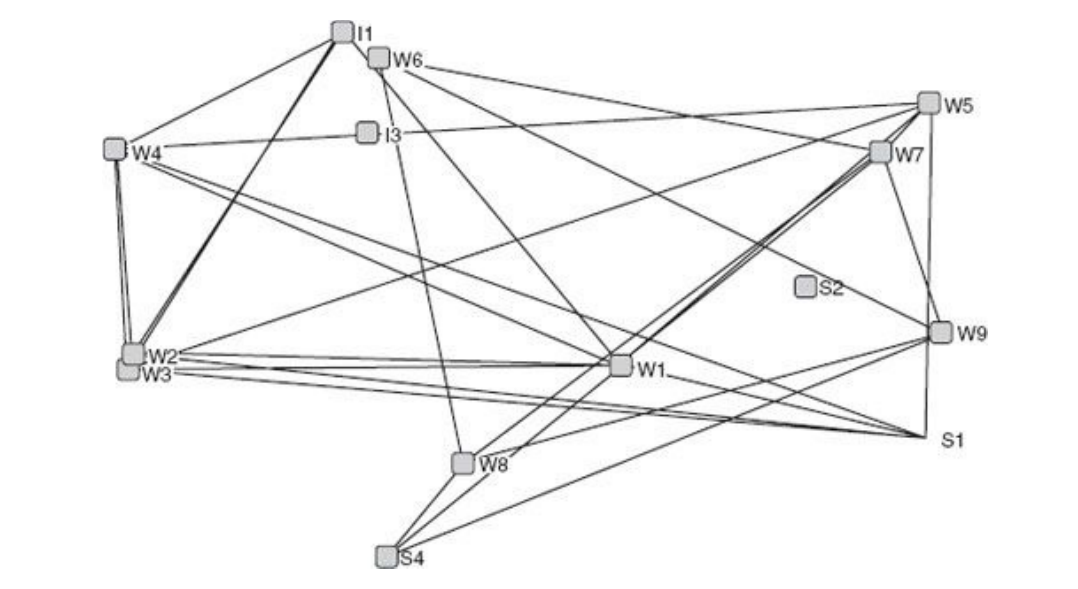
\includegraphics[width=\linewidth]{imagens/randomlayout.png}
        \caption{Aleatória} \label{fig:viza}
    \end{subfigure}
    %\\
    \vspace*{0.35cm}
    \begin{subfigure}{0.49\textwidth}
        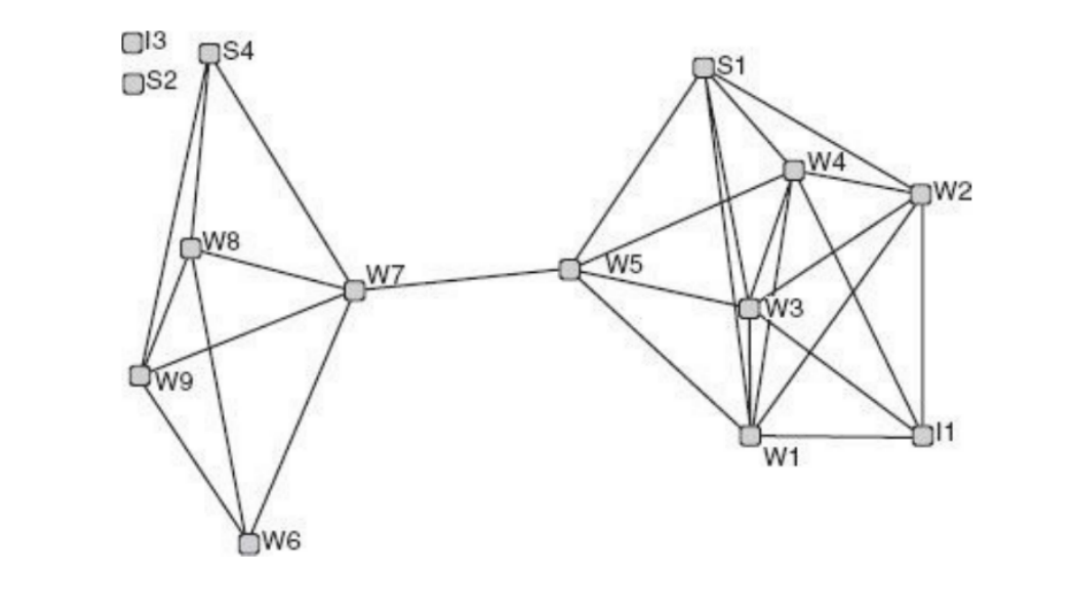
\includegraphics[width=\linewidth]{imagens/goodlayout2.png}
        \caption{Baseada em algoritmo} \label{fig:vizb}
    \end{subfigure}
    \vspace*{0.3cm}
    \caption{Comparação de visualizações de uma mesma rede complexa.}
    \label{fig:vizcomparison}
    \Fonte{Adaptado de \citeonline{Borgatti2013}.}
\end{figure}

% Referenciar PCA???
\citeonline{Borgatti2013} enumeram três estratégias para produzir visualizações de grafos: (i) gráfico de dispersão, onde atributos dos vértices são utilizados para determinar as suas coordenadas no plano cartesiano; (ii) redução de dimensionalidade, através de técnicas como análise de componentes principais, onde matrizes de associação entre vértices (contendo, por exemplo, distâncias ou correlações entre atributos) são mapeadas para coordenadas, aproximando os vértices de acordo com sua similaridade; e (iii) algoritmos de disposição de grafos, que são desenvolvidos especialmente para a tarefa de visualização e subdividem-se em vários tipos, como iterativos ou baseados em otimização matemática. \citeonline{Herman2000} fornecem uma revisão acerca de algoritmos de disposição, apontando suas características, vantagens e desvantagens.

Além disso, é possível aprimorar a interpretabilidade da visualização de grafos empregando artifícios como variação de cores, formas, tamanhos e espessuras. Por exemplo, pode-se utilizar a centralidade (discutida na Seção \ref{sec:centrality}) de cada vértice para determinar seu tamanho, modificar a espessura das ligações de acordo com seu peso, utilizar setas para indicar a direção dos arcos, entre outras opções \cite{Borgatti2013}.

\subsection{Análise Estatística} \label{sec:correlation}

A visualização de grafos, apesar de ser uma ferramenta de análise poderosa, está restrita ao domínio qualitativo e, portanto, está sujeita a interpretações e questões subjetivas, especialmente ao levar-se em conta as incertezas envolvendo a disposição dos vértices. Sendo assim, abordagens quantitativas, que apropriam-se de métodos estatísticos clássicos, também angariam considerável interesse na comunidade científica, por serem capazes de fornecer uma perspectiva objetiva e confirmatória acerca dos dados sob análise \cite{Atieno2009,Borgatti2013}.

No entanto, técnicas estatísticas clássicas assumem que os dados apresentam algumas características que não estão presentes em redes sociais, como a independência entre observações (afinal, sabe-se que existem processos de influência entre atores, conforme comentado na Seção \ref{sec:socialinfluence}) e a existência de uma distribuição estatística subjacente. Sendo assim, torna-se necessário realizar adaptações destas técnicas, visando habilitar seu uso de forma adequada em grafos \cite{Borgatti2013}. Conforme descrito na Seção \ref{sec:analysis}, análises básicas tem como objetivo principal identificar relações entre variáveis; para tanto, utiliza-se principalmente testes de hipótese, métodos de regressão (como a regressão linear) e métricas de correlação (como a de Pearson) \cite{DeNooy2005,Borgatti2013}.

\citeonline{Borgatti2013} sugerem a utilização de um método conhecido como \emph{teste de permutação}, que consiste em uma extensão a testes estatísticos clássicos. Testes de permutação consideram todos os resultados possíveis de um experimento, produzindo amostras de maneira aleatória; posteriormente, compara-se o valor de correlação obtido da amostra original com a distribuição de correlações das amostras aleatórias geradas. Com isso, calcula-se a proporção de amostras aleatórias que apresentaram correlação igual ou superior à original. Caso esta proporção seja inferior a um valor predeterminado (geralmente 5\%), então define-se que a relação entre as variáveis sob investigação é estatisticamente significante.
% com isso, a necessidade de independência é anulada.

Além disso, a existência de dois tipos de componentes em grafos -- vértices e ligações -- faz com que seja necessário utilizar metodologias adequadas ao nível de análise pretendido, de acordo com a hipótese que deseja-se testar. \citeonline{Borgatti2013} enumeram quatro níveis: (i) monádico, onde relaciona-se variáveis pertencentes exclusivamente a vértices; (ii) diádico, onde a análise é realizada entre pares de vértices, considerando características dos laços (imediatos ou não); (iii) misto, onde busca-se associar variáveis monádicas com diádicas (por exemplo, centralidade com amizades); e (iv) global, onde analisa-se variáveis que dizem respeito ao grafo como um todo (por exemplo, densidade e modularidade).

Para os níveis monádicos e globais, pode-se empregar técnicas estatísticas naturalmente, bastando utilizá-las juntamente com testes de permutação. No entanto, análises envolvendo díades (níveis diádicos e mistos) apresentam dificuldades significativas, pois as variáveis assumem um formato matricial, seguindo a estrutura da matriz de adjacências (discutida na Seção \ref{fig:networkDefs}). Como as técnicas estatísticas clássicas estão aptas para lidar apenas com dados vetoriais, métodos específicos são necessários.

Um destes métodos é a família de estratégias QAP (\textit{Quadratic Assignment Procedure}\footnote{Tradução livre: Procedimento de Atribuição Quadrático}), desenvolvida por \citeonline{Hubert1976} e estudada no contexto de redes sociais por \citeonline{Krackhardt1988}. A técnica, disponível em forma de análise de correlação e regressão na aplicação UCINET \cite{Borgatti2013}, é capaz de inferir associações entre matrizes de dados, e portanto pode ser empregada em níveis de análise diádicos. No caso do nível misto, existem estratégias para converter o vetor de dados monádico em uma matriz, possibilitando aplicação da técnica QAP \cite{Borgatti2013}, sendo possível também converter a matriz de dados diádica em um vetor, permitindo o uso de técnicas clássicas \cite{Blansky2013}.

\subsection{SIENA} \label{sec:siena}

A metodologia SIENA (\textit{Simulation Investigation for Empirical Network Analysis}\footnote{Tradução livre: Investigação de Simulações para Análise Empírica de Redes}), proposta por \citeonline{Snijders2001}, consiste em uma abordagem baseada em atores voltada para a análise de dados de redes sociais coletados de forma longitudinal; ou seja, onde tem-se instâncias de uma mesma rede de indivíduos em diferentes pontos no tempo.

A metodologia, em linhas gerais, busca simular o comportamento de processos sociais reais através de uma cadeia de Markov de tempo contínuo, onde o único evento passível de ocorrência em cada instante da simulação é a formação ou rompimento de uma ligação entre um par de vértices. Sendo assim, o modelo busca decompôr as mudanças ocorridas na rede social de uma coleta de dados para a próxima em passos simples, de apenas um evento. A frequência de execução de passos na simulação é especificada por uma função, que consiste em um parâmetro do modelo \cite{Borgatti2013}.

Por se tratar de uma abordagem baseada em atores, a simulação realizada pelo SIENA tem como ponto chave o processo de decisão individual de cada de ator da rede social, onde a opção por formação ou rompimento de ligações é guiada por uma função de avaliação definida pelo analista. Esta função pode levar em consideração atributos monádicos, diádicos e globais; com isso, é possível extrair inferências acerca destas variáveis, tornando o modelo altamente flexível e aplicável a uma grande gama de contextos (exemplos incluem os trabalhos de \citeonline{Rambaran2017} e \citeonline{Gremmen2017}, descritos na próxima seção). Entretanto, devido à complexidade inerente ao processo de simulação, podem existir dificuldades no tocante à interpretação dos resultados produzidos pelo modelo \textit{(ibidem)}.

% provavelmente vai ter que mudar \ref{sec:rambaran}
% já mudei


